\chapter{Ergebnisse}

Sofern nicht anders erwähnt, beziehen sich die Laufzeiten auf Systeme mit zwei Intel Xeon Gold 6230 Prozessoren mit einer Taktrate von \SI{2.1}{\giga\hertz} und \SI{180}{\giga\byte} RAM.
Die Ergebnisse wurden auf verschiedenen, aber identisch ausgestatteten Systemen des BwUniCluster2.0 erzeugt.

\section{Untersuchung der Graphen}

Der Fokus dieser Arbeit liegt auf drei Sichtbarkeitsgraphen, die jeweils einen Ausschnitt der Ozeane repräsentieren.
Ihre Knoten liegen dabei auf den Küsten.
Für jeden dieser drei Sichtbarkeitsgraphen existiert zusätzlich eine Triangulierung, deren Abstände eine untere Schranke zu den Abständen der jeweiligen Sichtbarkeitsgraphen darstellen.
\autoref{table:input_graphs} listet die Anzahl der Kanten und Knoten der Graphen auf.
Die Graphen mit dem Präfix \emph{aegaeis} umfassen das Ägäische Meer, diejenigen mit \emph{medi} decken das Mittelmeer ab, und die mit \emph{pata} repräsentieren die Chilenischen Fjorde.
Graphen mit dem Suffix \emph{visibility} sind Sichtbarkeitsgraphen, mit \emph{graph} Triangulierungen.

Die untersuchten Graphen sind ungerichtet, werden jedoch im weiteren Verlauf dieser Arbeit als gerichtet betrachtet.
Insbesondere ist die in \autoref{table:input_graphs} aufgelistete Anzahl an Kanten gerichtet zu interpretieren, die ungerichtete Kante $\{a, b\}$ wird also doppelt gezählt als $(a, b)$ und $(b, a)$.

\begin{table}[h!]
  \centering
  \begin{tabular}{
      l % Graph
      S[table-format = 7.0] % Zeit
      S[table-format = 9.0] % Zeit
      S[table-format = 4.1] % Zeit
    }
    \toprule
    {Graph}            & {\# Knoten} & {\# Kanten} & {$\varnothing$ Grad}       \\ \midrule
    aegaeis-graph      & 524881      & 2795322     & \fpeval{2795322/524881}    \\
    aegaeis-visibility & 201040      & 310231834   & \fpeval{310231834/201040}  \\
    medi-graph         & 795606      & 4223566     & \fpeval{4223566/795606}    \\
    medi-visibility    & 310116      & 730772548   & \fpeval{730772548/310116}  \\
    pata-graph         & 2240339     & 11632900    & \fpeval{11632900/2240339}  \\
    pata-visibility    & 1002235     & 315653892   & \fpeval{315653892/1002235} \\ \bottomrule
  \end{tabular}
  \caption{Bearbeite Graphen}
  \label{table:input_graphs}
\end{table}

\subsection{Dijkstra}

Für die Berechnung des Speedups der angewendeten Methoden wurden für jeden Graphen \num{1000} sequentielle $s$-$t$-Dijkstra-Suchen ausgeführt und die durchschnittliche Laufzeit ermittelt.
Die ermittelten Zeiten für das Finden des $s$-$t$-Abstands sind in Tabelle \ref{fig:ergebnisse:dijkstra} dargestellt.
Aus den Ergebnissen geht hervor, dass die Dijkstra-Suchen auf den Sichtbarkeitsgraphen im Vergleich zu auf ihren Triangulierungen deutlich höhere Laufzeiten aufweisen.

Zusätzlich zur durchschnittlichen Dijkstra-Laufzeit wurden die Durchschnittswerte der Hop-Längen, des Dijkstra-Ranks und der Queue-Pops über \num{10000} parallele $s$-$t$-Dijkstra-Suchen ermittelt, um ein Verständnis für die Laufzeiten zu erlangen.
Der Dijkstra-Rank ist die Anzahl der expandierten Knoten zum Zeitpunkt der Expansion des Zielknotens, die Queue-Pops die Anzahl der aus der Prioritätswarteschlange der Dijkstra-Suche entnommen Knoten.
Es zeigte sich, dass die durchschnittliche Hop-Länge in den Sichtbarkeitsgraphen signifikant kürzer ist als in den Triangulierungen.
Obwohl die Sichtbarkeitsgraphen weniger Knoten aufweisen, ist die durchschnittliche Anzahl der Queue-Pops dennoch höher.

\begin{table}[h!]
  \centering
  \begin{tabular}{
      l % Graph
      S[table-format = 4.1] % Zeit
      S[table-format = 3.0] % hop-länge
      S[table-format = 7.0] % rank
      S[table-format = 7.0] % queue pops
    }
    \toprule
    {Graph}            & {$\varnothing$ $t({spd})$} & {$\varnothing$  Hop-Länge} & {$\varnothing$ Dijkstra-Rank} & {$\varnothing$ Queue-Pops} \\
                       & {(\si{\ms})}               &                            &                               &                            \\
    \midrule
    aegaeis-graph      & 60.281198                  & 215.7201                   & 260447.36                     & 325845.56                  \\
    aegaeis-visibility & 630.434928                 & 16.311                     & 98650.82                      & 517346.63                  \\
    medi-graph         & 87.08376                   & 340.445                    & 394855.78                     & 494553.97                  \\
    medi-visibility    & 1279.67479                 & 23.6149                    & 154092.42                     & 959206.4                   \\
    pata-graph         & 265.825771                 & 883.979                    & 1120841.9                     & 1387047.8                  \\
    pata-visibility    & 1017.695977                & 63.817                     & 498570.2                      & 2429689.8                  \\ \bottomrule
  \end{tabular}
  \caption{Kennwerte der Dijkstra Suchen}
  \label{fig:ergebnisse:dijkstra}
\end{table}

\subsection{Knotengrade}

Es wurde die Verteilung der Knotengrade untersucht, die resultierenden Histogramme sind in \autoref{ergebnisse:fig:degree_hist} dargestellt.
In allen untersuchten Sichtbarkeitsgraphen haben mindestens 90\% der Knoten einen Grad von weniger als \num{2000}.

\begin{figure}[p]
  \begin{subfigure}[b]{0.5\textwidth}
    \resizebox{\textwidth}{!}{%
      \begin{tikzpicture}
        \begin{axis}[
            tick align=outside,
            tick pos=left,
            xmin=-698, xmax=14702,
            xtick style={color=black},
            xtick distance=2000,
            ymin=0, ymax=0.747618384401001,
            ytick style={color=black},
            ytick={0,0.1,0.2,0.3,0.4,0.5,0.6,0.7,0.8},
            yticklabels={0,10,20,30,40,50,60,70,80},
            xlabel={Knotengrad},
            ylabel={Anteil der Knoten (\%)}
          ]
          \draw[pattern=north east lines, pattern color=CadetBlue] (axis cs:2,0) rectangle (axis cs:2002,0.712017508953334);
          \draw[pattern=north east lines, pattern color=CadetBlue] (axis cs:2002,0) rectangle (axis cs:4002,0.194220055711032);
          \draw[pattern=north east lines, pattern color=CadetBlue] (axis cs:4002,0) rectangle (axis cs:6002,0.0606247512935969);
          \draw[pattern=north east lines, pattern color=CadetBlue] (axis cs:6002,0) rectangle (axis cs:8002,0.0205382013530728);
          \draw[pattern=north east lines, pattern color=CadetBlue] (axis cs:8002,0) rectangle (axis cs:10002,0.00766514126545947);
          \draw[pattern=north east lines, pattern color=CadetBlue] (axis cs:10002,0) rectangle (axis cs:12002,0.00397930760049903);
          \draw[pattern=north east lines, pattern color=CadetBlue] (axis cs:12002,0) rectangle (axis cs:14002,0.000955033824119655);
        \end{axis}
      \end{tikzpicture}
    }
    \caption{aegaeis-visibility}
  \end{subfigure}%
  \begin{subfigure}[b]{0.5\textwidth}
    \resizebox{\textwidth}{!}{%
      \begin{tikzpicture}
        \begin{axis}[
            tick align=outside,
            tick pos=left,
            xlabel={Knotengrad},
            xmin=-1198, xmax=25202,
            xtick distance=4000,
            xtick style={color=black},
            ylabel={Anteil der Knoten (\%)},
            ymin=0, ymax=0.637890337808629,
            ytick style={color=black},
            ytick={0,0.1,0.2,0.3,0.4,0.5,0.6,0.7},
            yticklabels={0,10,20,30,40,50,60,70}
          ]
          \draw[pattern=north east lines, pattern color=CadetBlue] (axis cs:2,0) rectangle (axis cs:2002,0.60751460743679);
          \draw[pattern=north east lines, pattern color=CadetBlue] (axis cs:2002,0) rectangle (axis cs:4002,0.207212784893063);
          \draw[pattern=north east lines, pattern color=CadetBlue] (axis cs:4002,0) rectangle (axis cs:6002,0.0905080679486225);
          \draw[pattern=north east lines, pattern color=CadetBlue] (axis cs:6002,0) rectangle (axis cs:8002,0.0423164235317719);
          \draw[pattern=north east lines, pattern color=CadetBlue] (axis cs:8002,0) rectangle (axis cs:10002,0.0196700589456533);
          \draw[pattern=north east lines, pattern color=CadetBlue] (axis cs:10002,0) rectangle (axis cs:12002,0.0103219440467273);
          \draw[pattern=north east lines, pattern color=CadetBlue] (axis cs:12002,0) rectangle (axis cs:14002,0.00818403436132265);
          \draw[pattern=north east lines, pattern color=CadetBlue] (axis cs:14002,0) rectangle (axis cs:16002,0.00425647177184629);
          \draw[pattern=north east lines, pattern color=CadetBlue] (axis cs:16002,0) rectangle (axis cs:18002,0.00420165357478464);
          \draw[pattern=north east lines, pattern color=CadetBlue] (axis cs:18002,0) rectangle (axis cs:20002,0.00342452501643997);
          \draw[pattern=north east lines, pattern color=CadetBlue] (axis cs:20002,0) rectangle (axis cs:22002,0.00236363167330556);
          \draw[pattern=north east lines, pattern color=CadetBlue] (axis cs:22002,0) rectangle (axis cs:24002,2.57967986172503e-05);
        \end{axis}
      \end{tikzpicture}%
    }%
    \caption{medi-visibility}%
  \end{subfigure}%
  \par\bigskip
  \begin{subfigure}[b]{0.5\textwidth}%
    \resizebox{\textwidth}{!}{%
      \begin{tikzpicture}%
        \begin{axis}[
            tick align=outside,
            tick pos=left,
            xlabel={Knotengrad},
            ylabel={Anteil der Knoten (\%)},
            xmin=-998, xmax=21002,
            xtick style={color=black},
            y grid style={darkgray176},
            xtick distance=4000,
            ymin=0, ymax=1.02857224104146,
            ytick style={color=black},
            ytick={0,0.2,0.4,0.6,0.8,1,1.2},
            yticklabels={0,20,40,60,80,100,120}
          ]
          \draw[pattern=north east lines, pattern color=CadetBlue] (axis cs:2,0) rectangle (axis cs:2002,0.979592610515676);
          \draw[pattern=north east lines, pattern color=CadetBlue] (axis cs:2002,0) rectangle (axis cs:4002,0.0169022235303201);
          \draw[pattern=north east lines, pattern color=CadetBlue] (axis cs:4002,0) rectangle (axis cs:6002,0.00222602483448042);
          \draw[pattern=north east lines, pattern color=CadetBlue] (axis cs:6002,0) rectangle (axis cs:8002,0.000968834654540784);
          \draw[pattern=north east lines, pattern color=CadetBlue] (axis cs:8002,0) rectangle (axis cs:10002,0.000297335455255565);
          \draw[pattern=north east lines, pattern color=CadetBlue] (axis cs:10002,0) rectangle (axis cs:12002,3.99107993631631e-06);
          \draw[pattern=north east lines, pattern color=CadetBlue] (axis cs:12002,0) rectangle (axis cs:14002,0);
          \draw[pattern=north east lines, pattern color=CadetBlue] (axis cs:14002,0) rectangle (axis cs:16002,9.97769984079078e-07);
          \draw[pattern=north east lines, pattern color=CadetBlue] (axis cs:16002,0) rectangle (axis cs:18002,3.99107993642733e-06);
          \draw[pattern=north east lines, pattern color=CadetBlue] (axis cs:18002,0) rectangle (axis cs:20002,3.99107993631631e-06);
        \end{axis}

      \end{tikzpicture}
    }
    \caption{pata-visibility}
  \end{subfigure}
  \caption{Verteilung der Kantengrade}
  \label{ergebnisse:fig:degree_hist}
\end{figure}

Als Indikator dafür, wie stark sich die Graphen kontrahieren lassen, wurde die Summe der quadratischen Knotengrade berechnet, diese sind in \autoref{table:sum_quad_degree} aufgelistet.
Bei den Sichtbarkeitsgraphen ist die Summe jeweils um mehrere Größenordnungen größer als bei ihren Triangulierungen, was darauf hindeutet, dass die Kontraktion dieser Graphen deutlich rechenintensiver sein dürfte.

\begin{table}[ht]
  \centering
  \begin{tabular}{
      l % Graph
      S[table-format = 13.0] % Zeit
    }
    \toprule
    {Graph}            & {$\sum_{v \in V} (\text{Grad}(v))^2$} \\
    \midrule
    aegaeis-graph      & 16024918                              \\
    aegaeis-visibility & 1153579966074                         \\
    medi-graph         & 24163472                              \\
    medi-visibility    & 4667069733248                         \\
    pata-graph         & 65662096                              \\
    pata-visibility    & 426189267238                          \\
    \bottomrule
  \end{tabular}
  \caption{Summe quadratischer Knotengrade}
  \label{table:sum_quad_degree}
\end{table}

\section{Graphen-Kontraktion}\label{section:ch_graph_kontraktion}

Es wurde versucht, die bearbeiteten Graphen mit einem eigens für die Arbeit entwickelten Programm zu kontrahieren.
Die Reihenfolge der Knoten-Kontraktionen wurde durch die Kanten-Differenz mit Lazy-Popping bestimmt.

Während es bei den triangulierten Graphen möglich war, einen Contracted-Graph zu erstellen, musste die Erstellung bei den Sichtbarkeitsgraphen nach drei Tagen abgebrochen werden, da in diesem Zeitraum nicht einmal alle initialen Kanten-Differenzen berechnet werden konnten.
Die Ergebnisse für die triangulierten Graphen sind in \autoref{fig:ergebnisse:ch_graph_kontraktion_triangulierungen} dargestellt, die Zeiten wurden über \num{100000} sequentielle $s$-$t$-Anfragen ermittelt.

\begin{table}[h!]
  \centering
  \begin{tabular}{
      l % Graph
      r % Erstellung
      S[table-format = 1.2] % Abkürzungen/Katen
      S[table-format = 9.0] % average time spd
      S[table-format = 4.0] % speedup
    }
    \toprule
    {Graph}       & {Erstellung} & {$\frac{\text{Abkürzungen} (C)}{\text{Kanten} (G)}$} & {$\varnothing$ $t({spd})$} & {Speedup}                          \\
    {}            & {}           & {}                                                   & {(\si{\us})}               & {}                                 \\
    \midrule
    aegaeis-graph & 2m 22s       & \fpeval{3253976/2795322}                             & 371.784                    & \fpeval{(60.281198*1000)/371.784}  \\
    medi-graph    & 3m 17s       & \fpeval{4845458/4223566}                             & 400.372                    & \fpeval{(87.08376*1000)/400.372}   \\
    pata-graph    & 9m 54s       & \fpeval{14187336/11632900}                           & 439.855                    & \fpeval{(265.825771*1000)/439.855} \\  \bottomrule
  \end{tabular}
  \caption{Kennwerte der Graphen-Kontraktion der triangulierten Graphen}
  \label{fig:ergebnisse:ch_graph_kontraktion_triangulierungen}
\end{table}

Basierend auf den Contracted-Graphen der Triangulierungen wurde für diese jeweils ein Hub-Graph durch Merging erstellt.
Die Ergebnisse hierfür sind in \autoref{fig:ergebnisse:hl_graph_kontraktion_triangulierungen} aufgelistet, die Zeiten wurden über \num{10000000} sequentielle $s$-$t$-Anfragen gebildet.

\begin{table}[h!]
  \centering
  \begin{tabular}{
      l % Graph
      r % Erstellung
      S[table-format = 3.0] % label
      S[table-format = 3.2] % average time spd
      S[table-format = 6.] % speedup
      S[table-format = 3.2] % average time sp
    }
    \toprule
    {Graph}       & {Erstellung}     & {$\varnothing$ $\abs{\text{Label}}$} & {$\varnothing$ $t({spd})$} & {Speedup}                        & {$\varnothing$ $t({spd})$} \\
    {}            & {}               & {}                                   & {(\si{\us})}               & {}                               & {(\si{\us})}               \\
    \midrule
    aegaeis-graph & 7m 11s           & 129.39623648026887                   & 1.436                      & \fpeval{(60.281198*1000)/1.436}  & 47.296                     \\
    medi-graph    & 9m \phantom{0}1s & 136.9877037126417                    & 1.454                      & \fpeval{(87.08376*1000)/1.454}   & 71.087                     \\
    pata-graph    & 29m 45s          & 133.48887779929734                   & 1.451                      & \fpeval{(265.825771*1000)/1.451} & 209.984                    \\
    \bottomrule
  \end{tabular}
  \caption{Kennwerte des Hierarchical Hub Labeling der triangulierten Graphen}
  \label{fig:ergebnisse:hl_graph_kontraktion_triangulierungen}
\end{table}

Als zusätzlicher Referenzpunkt zur Beurteilung der Qualität der erzeugten Contracted-Graphen sowie der dafür benötigten Zeit wurde ein externes Programm verwendet, um ebenfalls Contracted-Graphen zu erstellen.
Die Ergebnisse hierfür sind in \autoref{fig:ergebnisse:fmi_ch_graph_kontraktion_triangulierungen} aufgelistet.

Da dieses Programm ein anderes Speicherformat verwendet, konnten die Anfragezeiten nicht ermittelt werden.
Es kontrahierte im Vergleich zum in dieser Arbeit verwendeten Programm schneller, fügte jedoch mehr Abkürzungen ein.
Das Programm kontrahiert mehrere Knoten gleichzeitig, indem es \emph{unabhängige Teilmengen} von Knoten identifiziert, was eine effizientere parallele Verarbeitung ermöglicht \cite{vetter2009parallel}.
Angesichts des hohen durchschnittlichen Knotengrades der Sichtbarkeitsgraphen ist anzunehmen, dass nur wenige und kleine unabhängige Teilmengen existieren.
Dies schränkt den Nutzen der parallelen Kontraktion erheblich ein.
Auch dieses Programm konnte nach drei Tagen Laufzeit keine Ergebnisse liefern.

\begin{table}[h!]
  \centering
  \begin{tabular}{
      l % Graph
      r % Erstellung
      S[table-format = 1.2] % Abkürzungen/Katen
      S[table-format = 9.0] % average time spd
      S[table-format = 4.0] % speedup
    }
    \toprule
    {Graph}       & {Erstellung} & {$\frac{\text{Abkürzungen} (C)}{\text{Kanten} (G)}$} \\
    {}            & {(min)}      & {}                                                   \\
    \midrule
    aegaeis-graph & 22s          & \fpeval{(5446922-(2795322/2))/2795322}               \\
    medi-graph    & 34s          & \fpeval{(8156314-(4223566/2))/4223566}               \\
    pata-graph    & 1m 48s       & \fpeval{(23557322-(11632900/2))/11632900}            \\  \bottomrule
  \end{tabular}
  \caption{Kennwerte der Graphen-Kontraktion mit einem anderen Programm}
  \label{fig:ergebnisse:fmi_ch_graph_kontraktion_triangulierungen}
\end{table}

\subsection{Kontraktion mit oberer Schranke}\label{subsection:kontraktion_oberere_schranke}

Für die Untersuchung, ob sich die Kontraktion mit oberer Schranke auf die Graphen anwenden lässt, wurde von vornherein nur die Top-Down-Kontraktion untersucht, da die Bottom-Up-Kontraktion als zu rechenintensiv erschien.
Falls die Top-Down-Kontraktion anwendbar ist, könnte im nächsten Schritt die Bottom-Up-Kontraktion untersucht werden.

Für jeden Graphen wurde ein Hitting-Set aus \num{100000} zufällig generierten Pfaden erstellt.
Die Knoten, die Teil des Hitting-Sets waren, wurden nach der Iteration, in der sie ausgewählt wurden, sortiert.
Die übrigen Knoten wurden angehängt und entsprechend der Anzahl der kürzesten Pfade, auf denen sie lagen, sortiert.
Diese Anordnung wurde als level-to-vertex-Funktion verwendet:
Zuerst wurden die Knoten, die nicht Teil des Hitting-Sets sind, kontrahiert und anschließend die des Hitting-Sets.

\subsubsection{Triviale Heuristik}

Die Kontraktion mit der trivialen Heuristik als oberer Schranke ließ sich nicht auf die Sichtbarkeitsgraphen anwenden, da zu viele Abkürzungen eingefügt wurden und das Programm bereits nach wenigen Knoten-Kontraktionen aufgrund eines Speichermangels auf mit \SI{180}{\giga\byte} RAM ausgestatteten Computern abbrach.
Der Verlauf der Anzahl der Kanten des Graphs während der Kontraktion ist in \autoref{img:ergebnisse:all_in} abgebildet.

Obwohl für diese Arbeit auch Computer mit \SI{3}{\tera\byte} RAM  zur Verfügung standen, wurde das Experiment auf diesen nicht wiederholt, da die Anzahl der Kanten zu stark anstieg, um sinnvolle Ergebnisse erwarten zu können.

\begin{figure}[p]% Die Daten in den .csv Dateien sind gelippt auf 100. pgf hat Probleme mit zu großen Zahlen.
  \begin{subfigure}[b]{0.5\textwidth}
    \begin{tikzpicture}
      \begin{axis}[
          scale only axis, % The height and width argument only apply to the actual axis
          height=5cm,
          width=6cm,
          xlabel={Knoten-Kontraktionen},
          ylabel={Kanten},
        ]
        \addplot+[mark=none] table [x expr=\coordindex, y=Kanten, col sep=comma] {data/trivialheuristic/aegaeis.csv};
      \end{axis}
    \end{tikzpicture}
    \caption{aegaeis-visibility}%
  \end{subfigure}%
  \begin{subfigure}[b]{0.5\textwidth}%
    \begin{tikzpicture}
      \begin{axis}[
          scale only axis, % The height and width argument only apply to the actual axis
          height=5cm,
          width=6cm,
          xlabel={Knoten-Kontraktionen},
          ylabel={Kanten},
        ]
        \addplot+[mark=none] table [x expr=\coordindex, y=Kanten, col sep=comma] {data/trivialheuristic/medi.csv};
      \end{axis}
    \end{tikzpicture}
    \caption{medi-visibility}%
  \end{subfigure}%
  \par%
  \begin{subfigure}[b]{0.5\textwidth}%
    \begin{tikzpicture}
      \begin{axis}[
          scale only axis, % The height and width argument only apply to the actual axis
          height=5cm,
          width=6cm,
          xlabel={Knoten-Kontraktionen},
          ylabel={Kanten},
        ]
        \addplot+[mark=none] table [x expr=\coordindex, y=Kanten, col sep=comma] {data/trivialheuristic/pata.csv};
      \end{axis}
    \end{tikzpicture}
    \caption{pata-visibility}
  \end{subfigure}
  \caption{Graphen-Kontraktion mit oberer Schrank durch Triviale Heuristik}
  \label{img:ergebnisse:all_in}
\end{figure}

\subsubsection{Hubs, Vereinfachter Graph}


Die Abstände in triangulierten Graphen stellen, wie in \autoref{chapter:kontraktion} beschrieben, eine obere Schranke für die Abstände in Sichtbarkeitsgraphen dar.
Um den Fehler dieser Schranke zu quantifizieren, wurden die Abstände von einer \num{1000000} $s$-$t$-Paaren in den Sichtbarkeitsgraphen analysiert.
Der dabei ermittelte durchschnittliche Fehler pro Hop-Länge ist in \autoref{img:ergebnisse:upper_bound} als Datenreihe $\triangle$ dargestellt.

Diese Abbildung zeigt auch den durchschnittlichen Fehler, der durch den Einsatz von $n \in \mathbb{N}$ Hubs entsteht, welche mithilfe eines Hitting-Sets über \num{100000} Pfade bestimmt wurden.
Hierfür wurde die Erstellung des Hitting-Sets nach $n$ Iterationen vorzeitig abgebrochen.
Zusätzlich wurde der Fehler visualisiert, der sich aus der Wahl der kleinsten oberen Schranke zwischen 80 Hubs und den triangulierten Graphen ergibt.
Wie erwartet war die Kombination des triangulierten Graphen mit den Hubs sehr erfolgreich; insbesondere bei größeren Hop-Längen ist der Fehler oberen Schranke sehr gering.

\begin{figure}[p]% Die Daten in den .csv Dateien sind gelippt auf 100. pgf hat Probleme mit zu großen Zahlen.
  \begin{subfigure}[b]{0.5\textwidth}
    \begin{tikzpicture}
      \begin{axis}[
          scale only axis, % The height and width argument only apply to the actual axis
          height=5cm,
          width=6cm,
          ymax=6,
          xlabel={Hop-Länge},
          ylabel={Fehler (\%)},
          legend style={at={(1,0.475)},anchor=east, nodes={scale=0.8, transform shape}}
        ]
        \addplot+[mark repeat=9] table [x=hops, y=simple_graph_upper_bound, col sep=comma] {data/bounds/aegaeis.csv};
        \addlegendentry{$\triangle$};

        \addplot+[mark repeat=9] table [x=hops, y=10, col sep=comma] {data/bounds/aegaeis.csv};
        \addlegendentry{10 Hubs};

        \addplot+[mark repeat=9] table [x=hops, y=20, col sep=comma] {data/bounds/aegaeis.csv};
        \addlegendentry{20 Hubs};

        \addplot+[mark repeat=9] table [x=hops, y=40, col sep=comma] {data/bounds/aegaeis.csv};
        \addlegendentry{40 Hubs};

        \addplot+[mark repeat=9] table [x=hops, y=80, col sep=comma] {data/bounds/aegaeis.csv};
        \addlegendentry{80 Hubs};

        \addplot+[mark repeat=9] table [x=hops, y=min_80_simple, col sep=comma] {data/bounds/aegaeis.csv};
        \addlegendentry{$\triangle$, 80 Hubs};
      \end{axis}
    \end{tikzpicture}
    \caption{aegaeis-visibility}
  \end{subfigure}%
  \begin{subfigure}[b]{0.5\textwidth}
    \begin{tikzpicture}
      \begin{axis}[
          scale only axis, % The height and width argument only apply to the actual axis
          height=5cm,
          width=6cm,
          ymax=6,
          xlabel={Hop-Länge},
          ylabel={Fehler (\%)},
          legend style={at={(1,0.475)},anchor=east, nodes={scale=0.8, transform shape}}
        ]
        \addplot+[mark repeat=12] table [x=hops, y=simple_graph_upper_bound, col sep=comma] {data/bounds/medi.csv};
        \addlegendentry{$\triangle$};

        \addplot+[mark repeat=12] table [x=hops, y=10, col sep=comma] {data/bounds/medi.csv};
        \addlegendentry{10 Hubs};

        \addplot+[mark repeat=12] table [x=hops, y=20, col sep=comma] {data/bounds/medi.csv};
        \addlegendentry{20 Hubs};

        \addplot+[mark repeat=12] table [x=hops, y=40, col sep=comma] {data/bounds/medi.csv};
        \addlegendentry{40 Hubs};

        \addplot+[mark repeat=12] table [x=hops, y=80, col sep=comma] {data/bounds/medi.csv};
        \addlegendentry{80 Hubs};

        \addplot+[mark repeat=12] table [x=hops, y=min_80_simple, col sep=comma] {data/bounds/medi.csv};
        \addlegendentry{$\triangle$, 80 Hubs};
      \end{axis}
    \end{tikzpicture}
    \caption{medi-visibility}
  \end{subfigure}
  \par\bigskip
  \begin{subfigure}[b]{0.5\textwidth}
    \begin{tikzpicture}
      \begin{axis}[
          scale only axis, % The height and width argument only apply to the actual axis
          height=5cm,
          width=6cm,
          ymax=6,
          xlabel={Hop-Länge},
          ylabel={Fehler (\%)},
          legend style={at={(1,0.475)},anchor=east, nodes={scale=0.8, transform shape}}
        ]
        \addplot+[mark repeat=25] table [x=hops, y=simple_graph_upper_bound, col sep=comma] {data/bounds/pata.csv};
        \addlegendentry{$\triangle$};

        \addplot+[mark repeat=25] table [x=hops, y=10, col sep=comma] {data/bounds/pata.csv};
        \addlegendentry{10 Hubs};

        \addplot+[mark repeat=25] table [x=hops, y=20, col sep=comma] {data/bounds/pata.csv};
        \addlegendentry{20 Hubs};

        \addplot+[mark repeat=25] table [x=hops, y=40, col sep=comma] {data/bounds/pata.csv};
        \addlegendentry{40 Hubs};

        \addplot+[mark repeat=25] table [x=hops, y=80, col sep=comma] {data/bounds/pata.csv};
        \addlegendentry{80 Hubs};

        \addplot+[mark repeat=25] table [x=hops, y=min_80_simple, col sep=comma] {data/bounds/pata.csv};
        \addlegendentry{$\triangle$, 80 Hubs};
      \end{axis}
    \end{tikzpicture}
    \caption{pata-visibility}
  \end{subfigure}
  \caption{Fehler der oberen Schranken}
  \label{img:ergebnisse:upper_bound}
\end{figure}

Basierend auf dieser Untersuchung wurde versucht, die Sichtbarkeitsgraphen zu kontrahieren, wobei als obere Schranke ein Hub-Graph der Triangulierungen und 80 Hubs gewählt wurden.
Obwohl nach der vorhergehenden Analyse der Fehler der oberen Schranke als sehr klein betrachtet werden kann, war die Kontraktion nicht erfolgreich.

\autoref{fig:ergebnisse:hl_and_hubs} zeigt den Verlauf der Anzahl der Kanten während der Kontraktion.
Nach drei Tagen Rechenzeit waren die Graphen immer noch nicht kontrahiert, weshalb das Experiment abgebrochen wurde.
Die Anzahl der Kanten stieg während der Kontraktion wieder an, wenn auch langsamer als bei der trivialen Heuristik, wobei aegaeis-visibility und medi-visibility zum Zeitpunkt des Abbruchs den Höhepunkt der Anzahl der Kanten bereits erreicht hatten.

Damit die Kontraktion mit der oberen Schranke gelingen kann, muss der Fehler der oberen Schranke noch weiter reduziert werden, wobei dies nicht Teil dieser Arbeit ist.

\begin{figure}[p]% Die Daten in den .csv Dateien sind gelippt auf 100. pgf hat Probleme mit zu großen Zahlen.
  \begin{subfigure}[b]{0.5\textwidth}
    \centering
    \begin{tikzpicture}
      \begin{axis}[
          scale only axis, % The height and width argument only apply to the actual axis
          height=5cm,
          width=6cm,
          xlabel={Knoten-Kontraktionen (\%)},
          ylabel={Kanten},
        ]
        \addplot+[mark=none] table [x=x, y=matches, col sep=comma] {data/hlandhubs/aegaeis.csv};
      \end{axis}
    \end{tikzpicture}
    \caption{aegaeis-visibility}
  \end{subfigure}%
  \begin{subfigure}[b]{0.5\textwidth}
    \centering
    \begin{tikzpicture}
      \begin{axis}[
          scale only axis, % The height and width argument only apply to the actual axis
          height=5cm,
          width=6cm,
          xlabel={Knoten-Kontraktionen (\%)},
          ylabel={Kanten},
        ]
        \addplot+[mark=none] table [x=x, y=matches, col sep=comma] {data/hlandhubs/medi.csv};
      \end{axis}
    \end{tikzpicture}
    \caption{medi-visibility}
  \end{subfigure}
  \par\bigskip
  \begin{subfigure}[b]{0.5\textwidth}
    \centering
    \begin{tikzpicture}
      \begin{axis}[
          scale only axis, % The height and width argument only apply to the actual axis
          height=5cm,
          width=6cm,
          xlabel={Knoten-Kontraktionen (\%)},
          ylabel={Kanten},
        ]
        \addplot+[mark=none] table [x=x, y=matches, col sep=comma] {data/hlandhubs/pata.csv};
      \end{axis}
    \end{tikzpicture}
    \caption{pata-visibility}
  \end{subfigure}
  \caption{Graphen-Kontraktion mit oberer Schranke durch triangulierten Graph und Hubs}
  \label{fig:ergebnisse:hl_and_hubs}
\end{figure}

\section{PEOPLE}

Die in \autoref{chapter:people} vorgestellte Methode zur Berechnung von Contracted- und Hub-Graphen ließ sich auf die Sichtbarkeitsgraphen und ihre Triangulierungen anwenden.
Dabei konnten die Hub-Graphen entweder direkt durch PEOPLE erzeugt werden oder durch Merging eines mit CH-PEOPLE erstellten Contracted-Graphen.
Die vertex-to-level-Funktion wurde hierbei aus \autoref{subsection:kontraktion_oberere_schranke} übernommen.

\subsection{Contracted-Graph}

Durch die Berechnung aller Kanten, die von jedem Knoten im Downward- und Upward-Graphen ausgehen, konnte mit CH-PEOPLE sowohl für die Sichtbarkeitsgraphen als auch für deren Triangulierungen jeweils ein Contracted-Graph erstellt werden.
Die Kennzahlen zur Erzeugungs- und Anfragezeiten sind in \autoref{table:ergebnisse:people_ch_speedup} aufgeführt.

\begin{table}[h!]
  \centering
  \begin{tabular}{
      l % Graph
      r % S[table-format = 4.0] % Erstellung
      S[table-format = 1.2] % Abkürzungen/Katen
      S[table-format = 3.2] % average time spd
      S[table-format = 3.2] % speedup
    }
    \toprule
    {Graph}            & {Erstellung} & {$\frac{\text{Abkürzungen} (C)}{\text{Kanten} (G)}$} & {$\varnothing$ $t({spd})$} & {Speedup}                       \\
    {}                 & {}           & {}                                                   & {(\si{\ms})}               & {}                              \\ \midrule
    aegaeis-graph      & 20m          & \fpeval{12443056/2795322}                            & 2.290886                   & \fpeval{60.281198/2.290886}     \\
    aegaeis-visibility & 5h 53m       & \fpeval{214987558/310231834}                         & 408.948758                 & \fpeval{630.434928/408.948758}  \\
    medi-graph         & 38m          & \fpeval{20003908/4223566}                            & 3.38788                    & \fpeval{87.08376/3.38788}       \\
    medi-visibility    & 20h 52m      & \fpeval{468641256/730772544}                         & 832.555567                 & \fpeval{1279.67479/832.555567}  \\
    pata-graph         & 5h 42m       & \fpeval{70624466/11632900}                           & 10.16729                   & \fpeval{265.825771/10.16729}    \\
    pata-visibility    & 1d 20h 45m   & \fpeval{613324174/315653758}                         & 288.514849                 & \fpeval{1017.695977/288.514849} \\  \bottomrule
  \end{tabular}
  \caption{Kennwerte von mit CH-PEOPLE erzeugten Contracted-Graphen}
  \label{table:ergebnisse:people_ch_speedup}
\end{table}

Der Speedup der auf diese Weise für die Triangulierungen erzeugten Contracted-Graphen ist um Größenordnungen geringer als bei den durch Kontraktion erstellten Contracted-Graphen.
Zudem wurden jeweils mehr als dreimal so viele Abkürzungen hinzugefügt.
Im Verhältnis zur in die Erstellung der Contracted-Graphen investierten Rechenzeit erscheint der erzielte Speedup sehr gering.

Die zugrunde liegende vertex-to-level-Funktion weist jedoch eine begrenzte Qualität auf.
Es ist anzunehmen, dass durch den Einsatz einer besseren Funktion, welche durch ein Hitting-Set über mehr Pfade erstellt wurde, ein höherer Speedup hätte erzielt werden können.

\subsection{Hub Graph}

Aus den berechneten Contracted-Graphen konnten durch Merging als auch direkt durch PEOPLE Hub-Graphen erstellt werden.
Beide Wege erstellten nahezu identische Label und erreichten einen fünf- bis sechsstelligen Speedup.
Es galt zu klären, wie sich diese beiden Ansätze vergleichen lassen und wie schneller ein Hub-Graph generiert werden kann.

\subsubsection{Merging}

Ein zunächst verwendetes Programm, das einen Hub-Graphen aus einem Contracted-Graphen ohne Parallelisierung erzeugte, war nicht in der Lage, innerhalb von drei Tagen die Hub-Graphen der Sichtbarkeitsgraphen zu berechnen.
Der Grund hierfür liegt in der enormen Anzahl an Labels und Einträgen, die dabei zusammengeführt werden müssen: Ein Knoten der Contracted-Graphen der Sichtbarkeitsgraphen weist einen Grad im drei- bis vierstelligen Bereich auf, und für jeden dieser Nachbarn existiert ein Label, das gemerged werden muss.
Die Verwendung eines parallelen \emph{reduce}-Algorithmus führte zu den Ergebnissen in \autoref{table:ergebnisse:hl_ch_bruteforce},
dieser konnte für alle Graphen innerhalb von drei Tagen Hub-Graphen generieren.

\begin{table}[h!]
  \centering
  \begin{tabular}{ %MERGING
      l % Graph
      r % Erstellung
      S[table-format = 4.2] % label
      S[table-format = 2.2] % average time spd
      S[table-format = 6.0] % speedup
      S[table-format = 3.1] % average time sp
    }
    \toprule
    {Graph}            & {Erstellung}      & {$\varnothing$ $\abs{\text{Label}}$} & {$\varnothing$ $t({spd})$} & {Speedup$({spd})$}                 & {$\varnothing$ $t({sp})$} \\
    {}                 & {}                & {}                                   & {(\si{\us})}               & {}                                 & {(\si{\us})}              \\
    \midrule
    aegaeis-graph      & 12m               & 225.21998319619112                   & 1.617                      & \fpeval{(60.281198*1000)/1.617}    & 54.266                    \\
    aegaeis-visibility & 7h 35m            & 2447.866444488659                    & 9.382                      & \fpeval{(630.434928*1000)/9.382}   & 17.026                    \\
    medi-graph         & 19m               & 262.34248736183486                   & 1.777                      & \fpeval{(87.08376*1000)/1.777}     & 80.017                    \\
    medi-visibility    & 22h 18m           & 3528.6126965393596                   & 14.887                     & \fpeval{(1279.67479*1000)/14.887}  & 25.867                    \\
    pata-graph         & 1h 22m            & 451.8001829187458                    & 2.526                      & \fpeval{(265.825771*1000)/2.526}   & 264.981                   \\
    pata-visibility    & 14h \phantom{0}7m & 1823.062327697596                    & 16.862                     & \fpeval{(1017.695977*1000)/16.862} & 26.942                    \\
    \bottomrule
  \end{tabular}
  \caption{Kennwerte von mit Merging erstellter Hub-Graphen. Die zugrundeliegenden Contracted-Graphen wurden mit CH-PEOPLE erzeugt.}
  \label{table:ergebnisse:hl_ch_bruteforce}
\end{table}


\subsubsection{PEOPLE}

Die Hub-Graphen wurden ebenfalls durch PEOPLE berechnet, die entsprechenden Werte sind in \autoref{table:ergebnisse:hl_bruteforce} aufgeführt.

\begin{table}[h!]
  \centering
  \begin{tabular}{ %MERGING
      l % Graph
      r % Erstellung
      S[table-format = 4.2] % label
      S[table-format = 2.2] % average time spd
      S[table-format = 6.] % speedup
      S[table-format = 3.1] % average time sp
    }
    \toprule
    {Graph}            & {Erstellung}         & {$\varnothing$ $\abs{\text{Label}}$} & {$\varnothing$ $t({spd})$} & {Speedup$({spd})$}                 & {$\varnothing$ $t({sp})$} \\
    {}                 & {}                   & {}                                   & {(\si{\us})}               & {}                                 & {(\si{\us})}              \\
    \midrule
    aegaeis-graph      & 1h 26m               & 225.18963155458096                   & 1.612                      & \fpeval{(60.281198*1000)/1.612}    & 53.997                    \\
    aegaeis-visibility & 5h 57m               & 2446.9511241543973                   & 9.595                      & \fpeval{(630.434928*1000)/9.595}   & 17.31                     \\
    medi-graph         & 3h 11m               & 262.32183266591755                   & 1.787                      & \fpeval{(87.08376*1000)/1.787}     & 81.234                    \\
    medi-visibility    & 21h 57m              & 3527.5645951837378                   & 13.506                     & \fpeval{(1279.67479*1000)/13.506}  & 26.671                    \\
    pata-graph         & 1d \phantom{0}4h 26m & 451.71017734369667                   & 2.512                      & \fpeval{(265.825771*1000)/2.512}   & 263.59                    \\
    pata-visibility    & 1d 20h 17m           & 1822.0561604813242                   & 16.635                     & \fpeval{(1017.695977*1000)/16.635} & 27.324                    \\
    \bottomrule
  \end{tabular}
  \caption{Kennwerte von mit PEOPLE erstellen Hub-Graphen}
  \label{table:ergebnisse:hl_bruteforce}
\end{table}

\subsubsection{Vergleich}

Da Hub-Graphen auf zwei Wegen erzeugt werden können, muss geklärt werden, welcher effizienter ist, wobei effizienter sich hierbei nur die Laufzeit, nicht auf andere Metriken bezieht.
Dafür wurde die Zeit für die Erstellung des Contracted-Graphen mit CH-PEOPLE zu der Zeit für das Mergen addiert und anschließend mit der Zeit für die direkte Erstellung eines Hub-Graphen mittels PEOPLE verglichen.
Die entsprechenden Werte sind in \autoref{table:ergebnisse:vergleich_was_schneller} dargestellt.

Es zeigt sich, dass es bei den Sichtbarkeitsgraphen schneller ist, direkt einen Hub-Graphen zu berechnen, während bei den triangulierten Graphen der Umweg über die Contracted-Graphen effizienter ist.

\begin{table}[h!]
  \centering
  \begin{tabular}{ %VERGLEICH
      l % Graph
      r
      r
    }
    \toprule
    {Graph}            & {CH-PEOPLE \& Merging} & {PEOPLE}             \\
    \midrule
    aegaeis-graph      & \B 32m                 & 1h 26m               \\
    aegaeis-visibility & 13h 28m                & \B 5h 57m            \\
    medi-graph         & \B 57m                 & 3h 11m               \\
    medi-visibility    & 1d 19h 10m             & \B 21h 57m           \\
    pata-graph         & \B 7h \phantom{0}4m    & 1d \phantom{0}4h 26m \\
    pata-visibility    & 2d 10h 52m             & \B 1d 20h 17m        \\  \bottomrule
  \end{tabular}
  \caption{Vergleich der benötigten Zeit zum Erstellen von Hub-Graphen}
  \label{table:ergebnisse:vergleich_was_schneller}
\end{table}

Wie in \autoref{subsection:people:label_size} erwähnt, können die durch PEOPLE erzeugten Labels kleiner sein als die durch Merging erzeugten, was auch hier der Fall ist.
Der Unterschied in Bezug auf die Labelgröße ist zwar nicht besonders groß, aber dennoch erkennbar.
Da sich die Labelgrößen unterscheiden ist auch anzunehmen, dass die kürzesten Pfade auf den bearbeiteten Graphen nicht eindeutig sind.

\subsection{Performance Overhead}

Die Erzeugung der ausgehenden Kanten im Contracted-Graph sowie der Labels im Hub-Graph erfolgt durch modifizierte Dijkstra-Suchen und beinhaltet zusätzlich unter anderem die Sammlung von Abkürzungen.
Zur Quantifizierung des zusätzlichen Rechenaufwands im Vergleich zu Dijkstra-Suchen wurden für jeden Graphen, bei jeweils \emph{10000} Knoten, zwei Dijkstra-Suchen zu allen anderen Knoten durchgeführt.
Die dafür benötigte Rechenzeit wurde anschließend auf die Gesamtzahl der Knoten im Graphen skaliert.
\autoref{table:ergebnisse:dijkstra_vs_ch_vs_hl} zeigt die erforderliche Zeit zur Erstellung eines Contracted- und eines Hub-Graphen im Verhältnis zu dieser skalierten Zeit.

Auffällig ist, dass die Zeit für die Konstruktion eines Contracted-Graphen für die Triangulierungen nur geringfügig kürzer ist als die für einen Hub-Graphen.
Dies deutet darauf hin, dass in den meisten Fällen die Suche nur spät gestoppt wurde.

\begin{table}[h!]
  \centering
  \begin{tabular}{ %VERGLEICH
      l % Graph
      r % Graph
      S[table-format = 1.3] % average time
      S[table-format = 1.3] % average time
    }
    \toprule
    {Graph}            & {Dijkstra} & {$\frac{\text{CH-PEOPLE}}{\text{Dijkstra}}$}   & {$\frac{\text{PEOPLE}}{\text{Dijkstra}}$}      \\ \midrule
    aegaeis-graph      & 46m        & \fpeval{(20)/(46)}                             & \fpeval{(1*60+26)/(46)}                        \\
    aegaeis-visibility & 5h 19m     & \fpeval{(5*60+53)/(5*60+19)}                   & \fpeval{(5*60+57)/(5*60+19)}                   \\
    medi-graph         & 1h 46m     & \fpeval{(38)/(1*60+46)}                        & \fpeval{(3*60+11)/(1*60+46)}                   \\
    medi-visibility    & 19h 51m    & \fpeval{(20*60+52)/(19*60+51)}                 & \fpeval{(21*60+57)/(19*60+51)}                 \\
    pata-graph         & 14h 55m    & \fpeval{(5*60+42)/(14*60+55)}                  & \fpeval{(1*24*60+4*60+26)/(14*60+55)}          \\
    pata-visibility    & 1d 12h 32m & \fpeval{(1*24*60+20*60+45)/(1*24*60+12*60+32)} & \fpeval{(1*24*60+20*60+17)/(1*24*60+12*60+32)} \\  \bottomrule
  \end{tabular}
  \caption{Vergleich Performance Overhead von CH-PEOPLE und PEOPLE}
  \label{table:ergebnisse:dijkstra_vs_ch_vs_hl}
\end{table}

Für die Triangulierungen der Sichtbarkeitsgraphen ist es deutlich effizienter, Contracted-Graphen zu erstellen, anstatt für jeden Knoten jeweils zwei Dijkstra-Suchen durchzuführen.
Das deutet darauf hin, dass die Dijkstra-Suchen häufig vorzeitig abgebrochen werden konnten.

Um dieses Verhalten besser zu verstehen, wurde die CH-PEOPLE Suche in aegaeis-graph näher untersucht.
\autoref{fig:ergebnisse:ch_people_suchbaum} zeigt einen Suchbaum der CH-PEOPLE Suche.
In der Abbildung repräsentieren schwarze Punkte die Köpfe von Upward-Kanten, deren Fuß sich im weißen Punkt befindet.
Die durchgezogenen Linien stellen Kanten zu \emph{lebendigen} Knoten dar, während die gestrichelten Linien Kanten zu Knoten zeigen, die nicht mehr lebendig sind.
Für den betrachteten Knoten wurde lediglich ein Bruchteil der insgesamt \num{524881} möglichen Knoten besucht, was die Effizienz der CH-PEOPLE verdeutlicht.

\begin{figure}[h!]
  \centering
  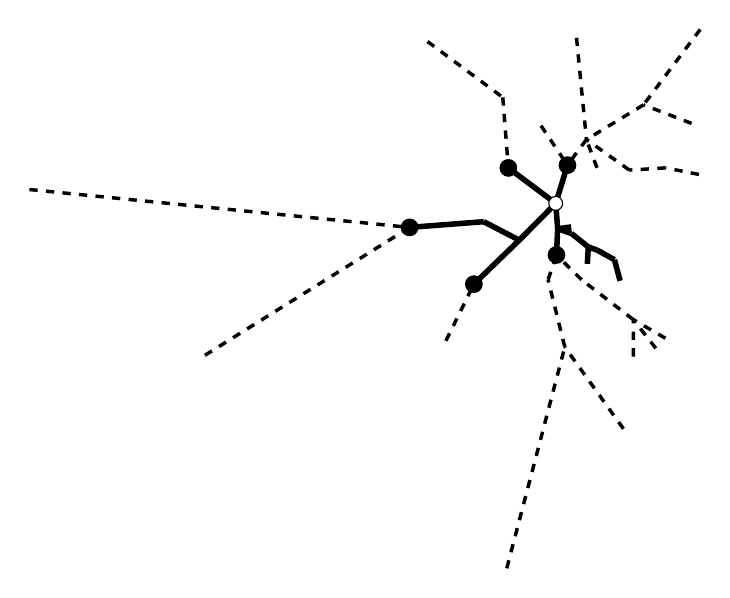
\begin{tikzpicture}[scale=1.5]
    \draw[line width=2] (4.456048319873318, 3.0900255391060227) edge (4.456048319873318, 3.0900255391060227);
    \draw[line width=2] (4.472612660101305, 2.8750437520344008) edge (4.456048319873318, 3.0900255391060227);
    \draw[line width=2] (4.587260603652865, 2.8905717642487616) edge (4.472612660101305, 2.8750437520344008);
    \draw[line width=2] (4.5889971877098645, 2.835738571829438) edge (4.472612660101305, 2.8750437520344008);
    \draw[line width=2] (4.555467757087328, 3.413754167559091) edge (4.456048319873318, 3.0900255391060227);
    \draw[line width=2] (4.46260040552211, 2.6534343050634845) edge (4.472612660101305, 2.8750437520344008);
    \draw[line width=2] (4.1474929335649335, 2.778701673953776) edge (4.456048319873318, 3.0900255391060227);
    \draw[line width=2] (4.05516128339265, 3.390271423153024) edge (4.456048319873318, 3.0900255391060227);
    \draw[line width=2] (4.731898018021141, 2.721123549710569) edge (4.5889971877098645, 2.835738571829438);
    \draw[line width=2] (4.808163001152366, 2.6938667891350576) edge (4.731898018021141, 2.721123549710569);
    \draw[line width=2] (4.7237357395051305, 2.577961439629206) edge (4.731898018021141, 2.721123549710569);
    \draw[line width=2] (4.9535573880579165, 2.6129010328780566) edge (4.808163001152366, 2.6938667891350576);
    \draw[line width=2] (3.846534022946102, 2.9349334463667276) edge (4.1474929335649335, 2.778701673953776);
    \draw[line width=2] (5.001135338416418, 2.434584433495246) edge (4.9535573880579165, 2.6129010328780566);
    \draw[line width=2] (3.7631245777735245, 2.4062629283591264) edge (4.1474929335649335, 2.778701673953776);
    \draw[line width=2] (3.2194560637723413, 2.886617108472933) edge (3.846534022946102, 2.9349334463667276);

    \draw[dashed,line width=1.25] (4.716279893465014, 3.6306879162957273) edge (4.555467757087328, 3.413754167559091);
    \draw[dashed,line width=1.25] (4.391620967473386, 2.443260777703671) edge (4.46260040552211, 2.6534343050634845);
    \draw[dashed,line width=1.25] (4.675476662781719, 2.4429315389880912) edge (4.46260040552211, 2.6534343050634845);
    \draw[dashed,line width=1.25] (4.331246054122673, 3.7480404128842792) edge (4.555467757087328, 3.413754167559091);
    \draw[dashed,line width=1.25] (4.805591520916153, 3.3906551281084774) edge (4.716279893465014, 3.6306879162957273);
    \draw[dashed,line width=1.25] (5.080161044919507, 3.3717017518306136) edge (4.716279893465014, 3.6306879162957273);
    \draw[dashed,line width=1.25] (4.007883808656132, 3.987747576108802) edge (4.05516128339265, 3.390271423153024);
    \draw[dashed,line width=1.25] (5.199329852951351, 3.9242600178816645) edge (4.716279893465014, 3.6306879162957273);
    \draw[dashed,line width=1.25] (4.5328890621807005, 1.8742850719746684) edge (4.391620967473386, 2.443260777703671);
    \draw[dashed,line width=1.25] (5.112877843259156, 2.1060471378532952) edge (4.675476662781719, 2.4429315389880912);
    \draw[dashed,line width=1.25] (5.385844366594839, 3.3906551281084774) edge (5.080161044919507, 3.3717017518306136);

    \draw[dashed,line width=1.25] (5.113512787335495, 1.7932534850537252) edge (5.112877843259156, 2.1060471378532952);
    \draw[dashed,line width=1.25] (5.3852877691412, 1.9481038374912885) edge (5.112877843259156, 2.1060471378532952);
    \draw[dashed,line width=1.25] (3.370595393721487, 4.4601669764603) edge (4.007883808656132, 3.987747576108802);
    \draw[dashed,line width=1.25] (5.029308443523917, 1.1816258114066613) edge (4.5328890621807005, 1.8742850719746684);
    \draw[dashed,line width=1.25] (3.5261803967035377, 1.9263597014372635) edge (3.7631245777735245, 2.4062629283591264);
    \draw[dashed,line width=1.25] (4.041647477097499, 0.0) edge (4.5328890621807005, 1.8742850719746684);
    \draw[dashed,line width=1.25] (0.0, 3.2073226303808156) edge (3.2194560637723413, 2.886617108472933);
    \draw[dashed,line width=1.25] (5.6063671485642175, 3.7671352248452195) edge (5.199329852951351, 3.9242600178816645);
    \draw[dashed,line width=1.25] (5.303556091896411, 1.8632888735496067) edge (5.112877843259156, 2.1060471378532952);
    \draw[dashed,line width=1.25] (5.679759184661748, 4.563044474936362) edge (5.199329852951351, 3.9242600178816645);
    \draw[dashed,line width=1.25] (5.668072671564062, 3.3352093179608744) edge (5.385844366594839, 3.3906551281084774);
    \draw[dashed,line width=1.25] (1.4858865913254249, 1.803766838849441) edge (3.2194560637723413, 2.886617108472933);
    \draw[dashed,line width=1.25] (4.6321645700874825, 4.491935662294821) edge (4.716279893465014, 3.6306879162957273);

    \filldraw (4.555467757087328, 3.413754167559091) circle (2pt);
    \filldraw (4.46260040552211, 2.6534343050634845) circle (2pt);
    \filldraw (4.05516128339265, 3.390271423153024) circle (2pt);
    \filldraw (3.7631245777735245, 2.4062629283591264) circle (2pt);
    \filldraw (3.2194560637723413, 2.886617108472933) circle (2pt);

    %\filldraw (4.456048319873318, 3.0900255391060227) circle (2pt);
    \node[circle,draw=black, fill=white, inner sep=0pt, minimum size=5pt] at (4.456048319873318, 3.0900255391060227) {};
  \end{tikzpicture}
  \caption{CH-PEOPLE Suchbaum auf aegaeis-graph}
  \label{fig:ergebnisse:ch_people_suchbaum}
\end{figure}

Nach der Untersuchung des einzelnen Suchvorganges wurden für aegaeis-graph für alle Knoten die bei der CH-PEOPLE-Suche gesehen Knoten erfasst.
Die Ergebnisse sind hierbei in \autoref{fig:ergebnisse:efficiency_ch_people} gelistet.
Bei \num{65}\% aller Suchen wurden weniger als \num{1}\% der \num{524881} Knoten gesehen.
Da die zugrunde vertex-to-level-Funktion auf einem Hitting-Set über nur \num{100000} Pfaden basiert, ist anzunehmen, dass durch eine bessere vertex-to-level-Funktion noch mehr Suchen \emph{lokaler} werden.

\begin{figure}[h!]%
  \centering
  \begin{tikzpicture}
    \begin{axis}[
        tick align=outside,
        tick pos=left,
        x grid style={darkgray176},
        xlabel={Gesehene Knoten (\%)},
        xmin=-5, xmax=105,
        xtick style={color=black},
        xtick={-20,0,20,40,60,80,100,120},
        xticklabels={\ensuremath{-}20,0,20,40,60,80,100,120},
        y grid style={darkgray176},
        ylabel={Anteil aller Suchen (\%)},
        ymin=0, ymax=0.68283477588288,
        ytick style={color=black},
        ytick={0,0.1,0.2,0.3,0.4,0.5,0.6,0.7},
        yticklabels={0,10,20,30,40,50,60,70}
      ]
      \draw[pattern=north east lines, pattern color=CadetBlue] (axis cs:0,0) rectangle (axis cs:1,0.650318834174171);
      \draw[pattern=north east lines, pattern color=CadetBlue] (axis cs:1,0) rectangle (axis cs:2,0.0261163959069088);
      \draw[pattern=north east lines, pattern color=CadetBlue] (axis cs:2,0) rectangle (axis cs:3,0.0121417997603392);
      \draw[pattern=north east lines, pattern color=CadetBlue] (axis cs:3,0) rectangle (axis cs:4,0.00762458538221844);
      \draw[pattern=north east lines, pattern color=CadetBlue] (axis cs:4,0) rectangle (axis cs:5,0.00591943697714958);
      \draw[pattern=north east lines, pattern color=CadetBlue] (axis cs:5,0) rectangle (axis cs:6,0.00413808082213352);
      \draw[pattern=north east lines, pattern color=CadetBlue] (axis cs:6,0) rectangle (axis cs:7,0.0037684732348896);
      \draw[pattern=north east lines, pattern color=CadetBlue] (axis cs:7,0) rectangle (axis cs:8,0.00317214759155249);
      \draw[pattern=north east lines, pattern color=CadetBlue] (axis cs:8,0) rectangle (axis cs:9,0.00266346086065494);
      \draw[pattern=north east lines, pattern color=CadetBlue] (axis cs:9,0) rectangle (axis cs:10,0.00286922178551252);
      \draw[pattern=north east lines, pattern color=CadetBlue] (axis cs:10,0) rectangle (axis cs:11,0.00370179145368577);
      \draw[pattern=north east lines, pattern color=CadetBlue] (axis cs:11,0) rectangle (axis cs:12,0.00250914016701176);
      \draw[pattern=north east lines, pattern color=CadetBlue] (axis cs:12,0) rectangle (axis cs:13,0.00217954164849032);
      \draw[pattern=north east lines, pattern color=CadetBlue] (axis cs:13,0) rectangle (axis cs:14,0.0018994781674343);
      \draw[pattern=north east lines, pattern color=CadetBlue] (axis cs:14,0) rectangle (axis cs:15,0.0015108186427033);
      \draw[pattern=north east lines, pattern color=CadetBlue] (axis cs:15,0) rectangle (axis cs:16,0.00119455648042266);
      \draw[pattern=north east lines, pattern color=CadetBlue] (axis cs:16,0) rectangle (axis cs:17,0.00104785656177409);
      \draw[pattern=north east lines, pattern color=CadetBlue] (axis cs:17,0) rectangle (axis cs:18,0.00181374444874349);
      \draw[pattern=north east lines, pattern color=CadetBlue] (axis cs:18,0) rectangle (axis cs:19,0.0011621681866949);
      \draw[pattern=north east lines, pattern color=CadetBlue] (axis cs:19,0) rectangle (axis cs:20,0.000874483930644265);
      \draw[pattern=north east lines, pattern color=CadetBlue] (axis cs:20,0) rectangle (axis cs:21,0.00245007916080286);
      \draw[pattern=north east lines, pattern color=CadetBlue] (axis cs:21,0) rectangle (axis cs:22,0.00248246745453029);
      \draw[pattern=north east lines, pattern color=CadetBlue] (axis cs:22,0) rectangle (axis cs:23,0.00250151939201715);
      \draw[pattern=north east lines, pattern color=CadetBlue] (axis cs:23,0) rectangle (axis cs:24,0.00151843941769825);
      \draw[pattern=north east lines, pattern color=CadetBlue] (axis cs:24,0) rectangle (axis cs:25,0.000830664474424814);
      \draw[pattern=north east lines, pattern color=CadetBlue] (axis cs:25,0) rectangle (axis cs:26,0.00121551361165795);
      \draw[pattern=north east lines, pattern color=CadetBlue] (axis cs:26,0) rectangle (axis cs:27,0.00128981616785639);
      \draw[pattern=north east lines, pattern color=CadetBlue] (axis cs:27,0) rectangle (axis cs:28,0.00128219539286178);
      \draw[pattern=north east lines, pattern color=CadetBlue] (axis cs:28,0) rectangle (axis cs:29,0.0039894757097364);
      \draw[pattern=north east lines, pattern color=CadetBlue] (axis cs:29,0) rectangle (axis cs:30,0.00172229514880695);
      \draw[pattern=north east lines, pattern color=CadetBlue] (axis cs:30,0) rectangle (axis cs:31,0.00136792911155248);
      \draw[pattern=north east lines, pattern color=CadetBlue] (axis cs:31,0) rectangle (axis cs:32,0.00192615087991577);
      \draw[pattern=north east lines, pattern color=CadetBlue] (axis cs:32,0) rectangle (axis cs:33,0.00115454741170029);
      \draw[pattern=north east lines, pattern color=CadetBlue] (axis cs:33,0) rectangle (axis cs:34,0.00117740973668445);
      \draw[pattern=north east lines, pattern color=CadetBlue] (axis cs:34,0) rectangle (axis cs:35,0.00108215004925027);
      \draw[pattern=north east lines, pattern color=CadetBlue] (axis cs:35,0) rectangle (axis cs:36,0.000988795555565081);
      \draw[pattern=north east lines, pattern color=CadetBlue] (axis cs:36,0) rectangle (axis cs:37,0.00104023578677936);
      \draw[pattern=north east lines, pattern color=CadetBlue] (axis cs:37,0) rectangle (axis cs:38,0.000685869749524892);
      \draw[pattern=north east lines, pattern color=CadetBlue] (axis cs:38,0) rectangle (axis cs:39,0.00248056226078164);
      \draw[pattern=north east lines, pattern color=CadetBlue] (axis cs:39,0) rectangle (axis cs:40,0.00177373538002135);
      \draw[pattern=north east lines, pattern color=CadetBlue] (axis cs:40,0) rectangle (axis cs:41,0.00124409151788818);
      \draw[pattern=north east lines, pattern color=CadetBlue] (axis cs:41,0) rectangle (axis cs:42,0.00176992499252404);
      \draw[pattern=north east lines, pattern color=CadetBlue] (axis cs:42,0) rectangle (axis cs:43,0.000956407261837544);
      \draw[pattern=north east lines, pattern color=CadetBlue] (axis cs:43,0) rectangle (axis cs:44,0.00181564964249215);
      \draw[pattern=north east lines, pattern color=CadetBlue] (axis cs:44,0) rectangle (axis cs:45,0.00151653422394948);
      \draw[pattern=north east lines, pattern color=CadetBlue] (axis cs:45,0) rectangle (axis cs:46,0.00239292334834229);
      \draw[pattern=north east lines, pattern color=CadetBlue] (axis cs:46,0) rectangle (axis cs:47,0.00170324321132043);
      \draw[pattern=north east lines, pattern color=CadetBlue] (axis cs:47,0) rectangle (axis cs:48,0.00103642539928195);
      \draw[pattern=north east lines, pattern color=CadetBlue] (axis cs:48,0) rectangle (axis cs:49,0.00108215004925039);
      \draw[pattern=north east lines, pattern color=CadetBlue] (axis cs:49,0) rectangle (axis cs:50,0.00138698104903923);
      \draw[pattern=north east lines, pattern color=CadetBlue] (axis cs:50,0) rectangle (axis cs:51,0.000621093162069708);
      \draw[pattern=north east lines, pattern color=CadetBlue] (axis cs:51,0) rectangle (axis cs:52,0.00110882276173196);
      \draw[pattern=north east lines, pattern color=CadetBlue] (axis cs:52,0) rectangle (axis cs:53,0.00302925806040166);
      \draw[pattern=north east lines, pattern color=CadetBlue] (axis cs:53,0) rectangle (axis cs:54,0.00227861172342159);
      \draw[pattern=north east lines, pattern color=CadetBlue] (axis cs:54,0) rectangle (axis cs:55,0.00165561336760311);
      \draw[pattern=north east lines, pattern color=CadetBlue] (axis cs:55,0) rectangle (axis cs:56,0.00112025392422388);
      \draw[pattern=north east lines, pattern color=CadetBlue] (axis cs:56,0) rectangle (axis cs:57,0.00205951444232344);
      \draw[pattern=north east lines, pattern color=CadetBlue] (axis cs:57,0) rectangle (axis cs:58,0.00140793818027474);
      \draw[pattern=north east lines, pattern color=CadetBlue] (axis cs:58,0) rectangle (axis cs:59,0.000691585330770961);
      \draw[pattern=north east lines, pattern color=CadetBlue] (axis cs:59,0) rectangle (axis cs:60,0.00104214098052813);
      \draw[pattern=north east lines, pattern color=CadetBlue] (axis cs:60,0) rectangle (axis cs:61,0.00138698104903912);
      \draw[pattern=north east lines, pattern color=CadetBlue] (axis cs:61,0) rectangle (axis cs:62,0.000502971149651588);
      \draw[pattern=north east lines, pattern color=CadetBlue] (axis cs:62,0) rectangle (axis cs:63,0.00190138336118284);
      \draw[pattern=north east lines, pattern color=CadetBlue] (axis cs:63,0) rectangle (axis cs:64,0.00123266035539626);
      \draw[pattern=north east lines, pattern color=CadetBlue] (axis cs:64,0) rectangle (axis cs:65,0.00440480794694864);
      \draw[pattern=north east lines, pattern color=CadetBlue] (axis cs:65,0) rectangle (axis cs:66,0.00320834627277755);
      \draw[pattern=north east lines, pattern color=CadetBlue] (axis cs:66,0) rectangle (axis cs:67,0.00282159194179543);
      \draw[pattern=north east lines, pattern color=CadetBlue] (axis cs:67,0) rectangle (axis cs:68,0.00207094560481547);
      \draw[pattern=north east lines, pattern color=CadetBlue] (axis cs:68,0) rectangle (axis cs:69,0.00175087305503696);
      \draw[pattern=north east lines, pattern color=CadetBlue] (axis cs:69,0) rectangle (axis cs:70,0.00218144684223898);
      \draw[pattern=north east lines, pattern color=CadetBlue] (axis cs:70,0) rectangle (axis cs:71,0.00120789283666334);
      \draw[pattern=north east lines, pattern color=CadetBlue] (axis cs:71,0) rectangle (axis cs:72,0.00121170322416064);
      \draw[pattern=north east lines, pattern color=CadetBlue] (axis cs:72,0) rectangle (axis cs:73,0.00120598764291446);
      \draw[pattern=north east lines, pattern color=CadetBlue] (axis cs:73,0) rectangle (axis cs:74,0.00148414593022206);
      \draw[pattern=north east lines, pattern color=CadetBlue] (axis cs:74,0) rectangle (axis cs:75,0.000682059362027698);
      \draw[pattern=north east lines, pattern color=CadetBlue] (axis cs:75,0) rectangle (axis cs:76,0.0010040371055543);
      \draw[pattern=north east lines, pattern color=CadetBlue] (axis cs:76,0) rectangle (axis cs:77,0.00308831906661078);
      \draw[pattern=north east lines, pattern color=CadetBlue] (axis cs:77,0) rectangle (axis cs:78,0.00205379886107737);
      \draw[pattern=north east lines, pattern color=CadetBlue] (axis cs:78,0) rectangle (axis cs:79,0.00400090687222843);
      \draw[pattern=north east lines, pattern color=CadetBlue] (axis cs:79,0) rectangle (axis cs:80,0.00244436357955691);
      \draw[pattern=north east lines, pattern color=CadetBlue] (axis cs:80,0) rectangle (axis cs:81,0.00208809234855345);
      \draw[pattern=north east lines, pattern color=CadetBlue] (axis cs:81,0) rectangle (axis cs:82,0.00528119707134167);
      \draw[pattern=north east lines, pattern color=CadetBlue] (axis cs:82,0) rectangle (axis cs:83,0.00305402557913448);
      \draw[pattern=north east lines, pattern color=CadetBlue] (axis cs:83,0) rectangle (axis cs:84,0.00230528443590305);
      \draw[pattern=north east lines, pattern color=CadetBlue] (axis cs:84,0) rectangle (axis cs:85,0.00455341305934576);
      \draw[pattern=north east lines, pattern color=CadetBlue] (axis cs:85,0) rectangle (axis cs:86,0.00329217479771948);
      \draw[pattern=north east lines, pattern color=CadetBlue] (axis cs:86,0) rectangle (axis cs:87,0.00422953012207028);
      \draw[pattern=north east lines, pattern color=CadetBlue] (axis cs:87,0) rectangle (axis cs:88,0.00162322507387547);
      \draw[pattern=north east lines, pattern color=CadetBlue] (axis cs:88,0) rectangle (axis cs:89,0.00502590110901857);
      \draw[pattern=north east lines, pattern color=CadetBlue] (axis cs:89,0) rectangle (axis cs:90,0.00425239244705433);
      \draw[pattern=north east lines, pattern color=CadetBlue] (axis cs:90,0) rectangle (axis cs:91,0.00176039902378056);
      \draw[pattern=north east lines, pattern color=CadetBlue] (axis cs:91,0) rectangle (axis cs:92,0.00117169415543839);
      \draw[pattern=north east lines, pattern color=CadetBlue] (axis cs:92,0) rectangle (axis cs:93,0.00560698520236602);
      \draw[pattern=north east lines, pattern color=CadetBlue] (axis cs:93,0) rectangle (axis cs:94,0.00772746584464701);
      \draw[pattern=north east lines, pattern color=CadetBlue] (axis cs:94,0) rectangle (axis cs:95,0.00288255814175331);
      \draw[pattern=north east lines, pattern color=CadetBlue] (axis cs:95,0) rectangle (axis cs:96,0.00501446994652632);
      \draw[pattern=north east lines, pattern color=CadetBlue] (axis cs:96,0) rectangle (axis cs:97,0.0057098656647947);
      \draw[pattern=north east lines, pattern color=CadetBlue] (axis cs:97,0) rectangle (axis cs:98,0.00931639743104651);
      \draw[pattern=north east lines, pattern color=CadetBlue] (axis cs:98,0) rectangle (axis cs:99,0.0207113612419031);
      \draw[pattern=north east lines, pattern color=CadetBlue] (axis cs:99,0) rectangle (axis cs:100,0.0650433145799436);
    \end{axis}
  \end{tikzpicture}
  \caption{Anteil der pro CH-PEOPLE Suche auf aegaeis-graph gesehenen Knoten}
  \label{fig:ergebnisse:efficiency_ch_people}
\end{figure}

\subsection{Vergleich verschiedener vertex-to-level-Funktionen}


Wie im  \autoref{chapter:people} erwähnt, lässt sich die durch eine vertex-to-level-Funktion induzierte durchschnittliche Labelgröße vorhersagen, indem für $n \in \mathbb{N}$ zufällig ausgewählte Knoten die Labels berechnet und von diesen die durchschnittliche Labelgröße bestimmt wird.
Diese Methode wurde verwendet, um verschiedene Funktionen zu vergleichen, die Ergebnisse sind in \autoref{table:ergebnisse:vtl_vergleich} gelistet.

Es wurden sechs vertex-to-level-Funktionen verglichen. Drei davon basierten auf einem Hitting-Set über \num{1000000}, wobei Knoten, die nicht im Hitting-Set enthalten waren, nach einer weiteren Metrik sortiert wurden. Diese war entweder eine zufällige Sortierung, eine Sortierung nach Grad (von klein nach groß) oder eine Sortierung danach, auf wie vielen kürzesten Pfaden die Knoten liegen.

Die anderen drei Funktionen waren eine zufällige Sortierung, eine Sortierung nach Grad (von klein nach groß) sowie die Übernahme der vertex-to-Level-Funktion, die durch die Graphen-Kontraktion der triangulierten Graphen entstand.
Letztere, in der Tabelle als $\triangle$ notiert, führte zu überraschend kleinen Labels.

\begin{table}[h!]
  \centering
  \begin{tabular}{l
      S[table-format = 6.0] % random
      S[table-format = 6.0] % random
      S[table-format = 6.0] % random
      S[table-format = 6.0] % random
      S[table-format = 6.0] % random
      S[table-format = 6.0] % random
    }
    \toprule
    Graph              & \multicolumn{3}{c}{Hitting-Set}   & {$\triangle$} & {Zufällig} & {Grad}   \\ \cline{2-4}
                       & {Zufällig} & {Hits}     & {Grad}  &               &            &          \\
    \midrule
    aegaeis-visibility & 1747.03    & \B 1420.17 & 1582.00 & 1473.27       & 17811.58   & 7420.85  \\
    medi-visibility    & 2487.06    & 2002.87    & 2422.12 & \B 1930.65    & 18700.13   & 12862.80 \\
    pata-visibility    & 1100.42    & \B 478.80  & 806.95  & 552.90        & 23690.52   & 10174.37 \\
    \bottomrule
  \end{tabular}
  \caption{Vorhergesagt durchschnittliche Labelgröße für verschiedene vertex-to-level-Funktion}
  \label{table:ergebnisse:vtl_vergleich}
\end{table}

\subsection{Große Hitting-Sets}

Mit den erzeugten Hub-Graphen wurden jeweils Hitting-Sets über \num{250000000} Pfade gebildet.
Die Knoten, die nicht enthalten waren, wurden danach sortiert, wie oft sie auf kürzesten Pfaden lagen, da dies nach \autoref{table:ergebnisse:vtl_vergleich} am Erfolgversprechenden erscheint.
Mit dieser vertex-to-level-Funktion wurde über \num{10000} Labels die durchschnittliche Labelgröße vorhergesagt, die Ergebnisse sind in \autoref{fig:ergebnisse:250_paths} aufgelistet.
Für die Sichtbarkeitsgraphen von aegaeis und medi ist die durchschnittliche Labelgröße kleiner als der ursprüngliche durchschnittliche Knotengrad.

\begin{table}[h!]
  \centering
  \begin{tabular}{ %VERGLEICH
      l % Graph
      r
      S[table-format = 4.1] % average time
    }
    \toprule
    {Graph}            & {Erstellung} & {$\varnothing$ $\abs{\text{Label}}$} \\ \midrule
    aegaeis-graph      & 6h 12m       & 90.8                                 \\
    aegaeis-visibility & 8h 11m       & 1309.8                               \\
    medi-graph         & 4h 47m       & 88.5                                 \\
    medi-visibility    & 12h 26m      & 1739.4                               \\
    pata-graph         & 2d 10h 37m   & 99.3                                 \\
    pata-visibility    & 9h 29m       & 424.1                                \\  \bottomrule
  \end{tabular}
  \caption{Vorhergesagt durchschnittliche Labelgröße für eine vertex-to-level-Funktion welche durch ein Hitting-Set über \num{250000000} Pfade induziert wurde}
  \label{fig:ergebnisse:250_paths}
\end{table}

Mit der entstandenen vertex-to-level-Funktion für aegaeis-graph wurde das der \autoref{fig:ergebnisse:efficiency_ch_people} zugrunde liegende Experiment wiederholt, wobei diesmal \num{86.7}\% aller Suchen weniger als 1\% aller Knoten sahen.
\autoref{fig:ergebnisse:new_efficiency_ch_people} zeigt die Abbildung mit den neuen Daten.

\begin{figure}
  \centering
  \begin{tikzpicture}
    \begin{axis}[
        tick align=outside,
        tick pos=left,
        x grid style={darkgray176},
        xlabel={Gesehene Knoten (\%)},
        xmin=-5, xmax=105,
        xtick style={color=black},
        xtick={-20,0,20,40,60,80,100,120},
        xticklabels={\ensuremath{-}20,0,20,40,60,80,100,120},
        y grid style={darkgray176},
        ylabel={Anteil aller Suchen (\%)},
        ymin=0, ymax=0.910038275342993,
        ytick style={color=black},
        ytick={0,0.1,0.2,0.3,0.4,0.5,0.6,0.7},
        yticklabels={0,10,20,30,40,50,60,70}
      ]
      \draw[pattern=north east lines, pattern color=CadetBlue] (axis cs:0,0) rectangle (axis cs:1,0.866703119374279);
      \draw[pattern=north east lines, pattern color=CadetBlue] (axis cs:1,0) rectangle (axis cs:2,0.0200159655236347);
      \draw[pattern=north east lines, pattern color=CadetBlue] (axis cs:2,0) rectangle (axis cs:3,0.00872769256270434);
      \draw[pattern=north east lines, pattern color=CadetBlue] (axis cs:3,0) rectangle (axis cs:4,0.00569271892105661);
      \draw[pattern=north east lines, pattern color=CadetBlue] (axis cs:4,0) rectangle (axis cs:5,0.00354556556629393);
      \draw[pattern=north east lines, pattern color=CadetBlue] (axis cs:5,0) rectangle (axis cs:6,0.00217382606724403);
      \draw[pattern=north east lines, pattern color=CadetBlue] (axis cs:6,0) rectangle (axis cs:7,0.00153939654893376);
      \draw[pattern=north east lines, pattern color=CadetBlue] (axis cs:7,0) rectangle (axis cs:8,0.00157369003640984);
      \draw[pattern=north east lines, pattern color=CadetBlue] (axis cs:8,0) rectangle (axis cs:9,0.00189185739243969);
      \draw[pattern=north east lines, pattern color=CadetBlue] (axis cs:9,0) rectangle (axis cs:10,0.00180421848000012);
      \draw[pattern=north east lines, pattern color=CadetBlue] (axis cs:10,0) rectangle (axis cs:11,0.00173372631129898);
      \draw[pattern=north east lines, pattern color=CadetBlue] (axis cs:11,0) rectangle (axis cs:12,0.00117359934918704);
      \draw[pattern=north east lines, pattern color=CadetBlue] (axis cs:12,0) rectangle (axis cs:13,0.000939260518099339);
      \draw[pattern=north east lines, pattern color=CadetBlue] (axis cs:13,0) rectangle (axis cs:14,0.00104785656177431);
      \draw[pattern=north east lines, pattern color=CadetBlue] (axis cs:14,0) rectangle (axis cs:15,0.0013622135303063);
      \draw[pattern=north east lines, pattern color=CadetBlue] (axis cs:15,0) rectangle (axis cs:16,0.00103452020553341);
      \draw[pattern=north east lines, pattern color=CadetBlue] (axis cs:16,0) rectangle (axis cs:17,0.00116026299294614);
      \draw[pattern=north east lines, pattern color=CadetBlue] (axis cs:17,0) rectangle (axis cs:18,0.000956407261837655);
      \draw[pattern=north east lines, pattern color=CadetBlue] (axis cs:18,0) rectangle (axis cs:19,0.00076779308071806);
      \draw[pattern=north east lines, pattern color=CadetBlue] (axis cs:19,0) rectangle (axis cs:20,0.000855431993157407);
      \draw[pattern=north east lines, pattern color=CadetBlue] (axis cs:20,0) rectangle (axis cs:21,0.000737309980739287);
      \draw[pattern=north east lines, pattern color=CadetBlue] (axis cs:21,0) rectangle (axis cs:22,0.00110691756798331);
      \draw[pattern=north east lines, pattern color=CadetBlue] (axis cs:22,0) rectangle (axis cs:23,0.000672533393284103);
      \draw[pattern=north east lines, pattern color=CadetBlue] (axis cs:23,0) rectangle (axis cs:24,0.000544885412122498);
      \draw[pattern=north east lines, pattern color=CadetBlue] (axis cs:24,0) rectangle (axis cs:25,0.00051821269964103);
      \draw[pattern=north east lines, pattern color=CadetBlue] (axis cs:25,0) rectangle (axis cs:26,0.000615377580823528);
      \draw[pattern=north east lines, pattern color=CadetBlue] (axis cs:26,0) rectangle (axis cs:27,0.000802086568194471);
      \draw[pattern=north east lines, pattern color=CadetBlue] (axis cs:27,0) rectangle (axis cs:28,0.000603946418331835);
      \draw[pattern=north east lines, pattern color=CadetBlue] (axis cs:28,0) rectangle (axis cs:29,0.000977364393072833);
      \draw[pattern=north east lines, pattern color=CadetBlue] (axis cs:29,0) rectangle (axis cs:30,0.00054679060587115);
      \draw[pattern=north east lines, pattern color=CadetBlue] (axis cs:30,0) rectangle (axis cs:31,0.000417237430961115);
      \draw[pattern=north east lines, pattern color=CadetBlue] (axis cs:31,0) rectangle (axis cs:32,0.000918303386863828);
      \draw[pattern=north east lines, pattern color=CadetBlue] (axis cs:32,0) rectangle (axis cs:33,0.00080780214944054);
      \draw[pattern=north east lines, pattern color=CadetBlue] (axis cs:33,0) rectangle (axis cs:34,0.000621093162069708);
      \draw[pattern=north east lines, pattern color=CadetBlue] (axis cs:34,0) rectangle (axis cs:35,0.000703016493262987);
      \draw[pattern=north east lines, pattern color=CadetBlue] (axis cs:35,0) rectangle (axis cs:36,0.000459151693431914);
      \draw[pattern=north east lines, pattern color=CadetBlue] (axis cs:36,0) rectangle (axis cs:37,0.000994511136811038);
      \draw[pattern=north east lines, pattern color=CadetBlue] (axis cs:37,0) rectangle (axis cs:38,0.000455341305934609);
      \draw[pattern=north east lines, pattern color=CadetBlue] (axis cs:38,0) rectangle (axis cs:39,0.000497255568405519);
      \draw[pattern=north east lines, pattern color=CadetBlue] (axis cs:39,0) rectangle (axis cs:40,0.000302925806040188);
      \draw[pattern=north east lines, pattern color=CadetBlue] (axis cs:40,0) rectangle (axis cs:41,0.000424858205955725);
      \draw[pattern=north east lines, pattern color=CadetBlue] (axis cs:41,0) rectangle (axis cs:42,0.000360081618500541);
      \draw[pattern=north east lines, pattern color=CadetBlue] (axis cs:42,0) rectangle (axis cs:43,0.000245769993579836);
      \draw[pattern=north east lines, pattern color=CadetBlue] (axis cs:43,0) rectangle (axis cs:44,0.000470582855924051);
      \draw[pattern=north east lines, pattern color=CadetBlue] (axis cs:44,0) rectangle (axis cs:45,0.000716352849503665);
      \draw[pattern=north east lines, pattern color=CadetBlue] (axis cs:45,0) rectangle (axis cs:46,0.000605851612080377);
      \draw[pattern=north east lines, pattern color=CadetBlue] (axis cs:46,0) rectangle (axis cs:47,0.000426763399704266);
      \draw[pattern=north east lines, pattern color=CadetBlue] (axis cs:47,0) rectangle (axis cs:48,0.000394375105976841);
      \draw[pattern=north east lines, pattern color=CadetBlue] (axis cs:48,0) rectangle (axis cs:49,0.000169562243632626);
      \draw[pattern=north east lines, pattern color=CadetBlue] (axis cs:49,0) rectangle (axis cs:50,0.000316262162280867);
      \draw[pattern=north east lines, pattern color=CadetBlue] (axis cs:50,0) rectangle (axis cs:51,0.000251485574825683);
      \draw[pattern=north east lines, pattern color=CadetBlue] (axis cs:51,0) rectangle (axis cs:52,0.000417237430961115);
      \draw[pattern=north east lines, pattern color=CadetBlue] (axis cs:52,0) rectangle (axis cs:53,0.000983079974318901);
      \draw[pattern=north east lines, pattern color=CadetBlue] (axis cs:53,0) rectangle (axis cs:54,0.000659197037043535);
      \draw[pattern=north east lines, pattern color=CadetBlue] (axis cs:54,0) rectangle (axis cs:55,0.000565842543357897);
      \draw[pattern=north east lines, pattern color=CadetBlue] (axis cs:55,0) rectangle (axis cs:56,0.000706826880760403);
      \draw[pattern=north east lines, pattern color=CadetBlue] (axis cs:56,0) rectangle (axis cs:57,0.000744930755734008);
      \draw[pattern=north east lines, pattern color=CadetBlue] (axis cs:57,0) rectangle (axis cs:58,0.000699206105765682);
      \draw[pattern=north east lines, pattern color=CadetBlue] (axis cs:58,0) rectangle (axis cs:59,0.000413427043463588);
      \draw[pattern=north east lines, pattern color=CadetBlue] (axis cs:59,0) rectangle (axis cs:60,0.000783034630707502);
      \draw[pattern=north east lines, pattern color=CadetBlue] (axis cs:60,0) rectangle (axis cs:61,0.00049725556840563);
      \draw[pattern=north east lines, pattern color=CadetBlue] (axis cs:61,0) rectangle (axis cs:62,0.00021528689360073);
      \draw[pattern=north east lines, pattern color=CadetBlue] (axis cs:62,0) rectangle (axis cs:63,0.00050297114965181);
      \draw[pattern=north east lines, pattern color=CadetBlue] (axis cs:63,0) rectangle (axis cs:64,0.00043628936844764);
      \draw[pattern=north east lines, pattern color=CadetBlue] (axis cs:64,0) rectangle (axis cs:65,0.000683964555776351);
      \draw[pattern=north east lines, pattern color=CadetBlue] (axis cs:65,0) rectangle (axis cs:66,0.000558221768363176);
      \draw[pattern=north east lines, pattern color=CadetBlue] (axis cs:66,0) rectangle (axis cs:67,0.000525833474635751);
      \draw[pattern=north east lines, pattern color=CadetBlue] (axis cs:67,0) rectangle (axis cs:68,0.000525833474635862);
      \draw[pattern=north east lines, pattern color=CadetBlue] (axis cs:68,0) rectangle (axis cs:69,0.000424858205955614);
      \draw[pattern=north east lines, pattern color=CadetBlue] (axis cs:69,0) rectangle (axis cs:70,0.00056012696211194);
      \draw[pattern=north east lines, pattern color=CadetBlue] (axis cs:70,0) rectangle (axis cs:71,0.000527738668384403);
      \draw[pattern=north east lines, pattern color=CadetBlue] (axis cs:71,0) rectangle (axis cs:72,0.000908777418120565);
      \draw[pattern=north east lines, pattern color=CadetBlue] (axis cs:72,0) rectangle (axis cs:73,0.000430573787201793);
      \draw[pattern=north east lines, pattern color=CadetBlue] (axis cs:73,0) rectangle (axis cs:74,0.0011412110554595);
      \draw[pattern=north east lines, pattern color=CadetBlue] (axis cs:74,0) rectangle (axis cs:75,0.00102689943053857);
      \draw[pattern=north east lines, pattern color=CadetBlue] (axis cs:75,0) rectangle (axis cs:76,0.000708732074509166);
      \draw[pattern=north east lines, pattern color=CadetBlue] (axis cs:76,0) rectangle (axis cs:77,0.000866863155649544);
      \draw[pattern=north east lines, pattern color=CadetBlue] (axis cs:77,0) rectangle (axis cs:78,0.000748741143231313);
      \draw[pattern=north east lines, pattern color=CadetBlue] (axis cs:78,0) rectangle (axis cs:79,0.000760172305723228);
      \draw[pattern=north east lines, pattern color=CadetBlue] (axis cs:79,0) rectangle (axis cs:80,0.00082875928067605);
      \draw[pattern=north east lines, pattern color=CadetBlue] (axis cs:80,0) rectangle (axis cs:81,0.000931639743104618);
      \draw[pattern=north east lines, pattern color=CadetBlue] (axis cs:81,0) rectangle (axis cs:82,0.00129362655535381);
      \draw[pattern=north east lines, pattern color=CadetBlue] (axis cs:82,0) rectangle (axis cs:83,0.000443910143442583);
      \draw[pattern=north east lines, pattern color=CadetBlue] (axis cs:83,0) rectangle (axis cs:84,0.000575368512101382);
      \draw[pattern=north east lines, pattern color=CadetBlue] (axis cs:84,0) rectangle (axis cs:85,0.000882104705638986);
      \draw[pattern=north east lines, pattern color=CadetBlue] (axis cs:85,0) rectangle (axis cs:86,0.000363892005997957);
      \draw[pattern=north east lines, pattern color=CadetBlue] (axis cs:86,0) rectangle (axis cs:87,0.00102689943053869);
      \draw[pattern=north east lines, pattern color=CadetBlue] (axis cs:87,0) rectangle (axis cs:88,0.000887820286884944);
      \draw[pattern=north east lines, pattern color=CadetBlue] (axis cs:88,0) rectangle (axis cs:89,0.00134697198031675);
      \draw[pattern=north east lines, pattern color=CadetBlue] (axis cs:89,0) rectangle (axis cs:90,0.00190709894242913);
      \draw[pattern=north east lines, pattern color=CadetBlue] (axis cs:90,0) rectangle (axis cs:91,0.000531549055881708);
      \draw[pattern=north east lines, pattern color=CadetBlue] (axis cs:91,0) rectangle (axis cs:92,0.000274347899810068);
      \draw[pattern=north east lines, pattern color=CadetBlue] (axis cs:92,0) rectangle (axis cs:93,0.00159083678014793);
      \draw[pattern=north east lines, pattern color=CadetBlue] (axis cs:93,0) rectangle (axis cs:94,0.000556316574614635);
      \draw[pattern=north east lines, pattern color=CadetBlue] (axis cs:94,0) rectangle (axis cs:95,0.000318167356029742);
      \draw[pattern=north east lines, pattern color=CadetBlue] (axis cs:95,0) rectangle (axis cs:96,0.000998321524308343);
      \draw[pattern=north east lines, pattern color=CadetBlue] (axis cs:96,0) rectangle (axis cs:97,0.00191090932992632);
      \draw[pattern=north east lines, pattern color=CadetBlue] (axis cs:97,0) rectangle (axis cs:98,0.00277586729182711);
      \draw[pattern=north east lines, pattern color=CadetBlue] (axis cs:98,0) rectangle (axis cs:99,0.0051059192464632);
      \draw[pattern=north east lines, pattern color=CadetBlue] (axis cs:99,0) rectangle (axis cs:100,0.015043409839579);
    \end{axis}
  \end{tikzpicture}
  \caption{Anteil der pro CH-PEOPLE Suche auf aegaeis-graph gesehenen Knoten}
  \label{fig:ergebnisse:new_efficiency_ch_people}
\end{figure}

\subsection{Weiterer Graph}

Als letzter Teil dieser Arbeit wurde mit \emph{planet-shrunk-visibility} ein Sichtbarkeitsgraph betrachtet, der analog zu den Sichtbarkeitsgraphenvon aegaeis, medi und pata konstruiert wurde, aber die gesamte Welt umfasst.
Er bestand aus \num{188030} Knoten und \num{173385124} Kanten.
Mittels PEOPLE konnte für ihn ein Hub-Graph erstellt werden, mit dem ein Speedup \num[round-mode=places,round-precision=0]{\fpeval{(529.377185*1000)/6.756}} im Vergleich zur Dijkstra erzielt wurde.

% \autoref{table:input_graphs_planet-shrunk-visibility} listet die Anzahl der Kanten und Knoten dieses Graphs auf.
% 
% \begin{table}[h!]
%   \centering
%   \begin{tabular}{
%       l % Graph
%       S[table-format = 7.0] % Zeit
%       S[table-format = 9.0] % Zeit
%       S[table-format = 4.1] % Zeit
%     }
%     \toprule
%     {Graph}                  & {\# Knoten} & {\# Kanten} & {$\varnothing$ Grad}      \\ \midrule
%     planet-shrunk-visibility & 188030      & 173385124   & \fpeval{173385124/188030} \\\bottomrule
%   \end{tabular}
%   \caption{Bearbeite Graphen}
%   \label{table:input_graphs_planet-shrunk-visibility}
% \end{table}
% 
% 
% \begin{table}[h!]
%   \centering
%   \begin{tabular}{
%       l % Graph
%       S[table-format = 4.1] % Zeit
%       S[table-format = 3.0] % hop-länge
%       S[table-format = 7.0] % rank
%       S[table-format = 7.0] % queue pops
%     }
%     \toprule
%     {Graph}                  & {$\varnothing$ $t({spd})$} & {$\varnothing$  Hop-Länge} & {$\varnothing$ Dijkstra-Rank} & {$\varnothing$ Queue-Pops} \\
%                              & {(\si{\ms})}               &                            &                               &                            \\
%     \midrule
%     planet-shrunk-visibility & 529.377185                 & 22.3786                    & 95053.74                      & 691017.2                   \\
%     \bottomrule
%   \end{tabular}
%   \caption{Kennwerte der Dijkstra Suchen}
%   \label{fig:ergebnisse:dijkstra_planet-shrunk-visibility}
% \end{table}
% 
% 
% Running `target/release/investigate_hl -h tests/data/planet-shrunk-vis-fixed-hl.bincode -n 10000000`
% average label size 1154.5453757379141
% shortcuts 63174890
% getting random paths distances takes 6.756µs on average
% getting random paths takes 11.242µs on average

% Is graph bidirectional? true
% non trivial vertices: 188030
% trivial: 188030
% average degree is 922.1135
% sum of squared degree 422505182196
% Values over 10000 parallel searches
% average path hops len 22.3786
% average dijkstra_rank 95053.74
% average queue pops 691017.2
% 2xDijsktra per node for all nodes would take 14810.959127085s
% Value over 100 sequential searches
% Average dijkstra duration for path creation is 573.84923ms
% Average dijkstra duration for path distance is 529.377185ms